\section{Internet of Things}
Internet of Things (IoT) \cite{BandaCM15} is an ecosystem of devices that are connected to the internet. The ‘thing’ can be anything from a heart monitor, an automobile, temperature sensor to a refrigerator. It includes any object that can transmit or receive data either directly or indirectly to the internet without manual assistance. The advent of wireless technology has lead to a rapid decrease in costs of such a system and increased the viability of a large deployment of IoT devices exponentially.

The devices are managed using an IoT platform which is a multi-layer technology that enables straightforward provisioning and management of connected devices. This has lead to IoT being widely used in connecting devices and collecting data information. The system is used to register their sensors, manage streams of data and handle configuration updates. Using a cloud-based service for the same greatly speeds up the development of applications and takes care of scalability and cross-device compatibility as well \cite{ref1.4}.

This connects your diverse hardware using a range of enterprise-grade connectivity options to huge data processing solutions, opening up a plethora of applications ranging from data collection to drone delivery networks to precision farming \cite{iotPAhighLevel}.

\section{Wireless Sensor Network}

A Wireless sensor network (WSN) refers to a group of spatially dispersed connected sensors that can be used for monitoring and recording the environmental conditions and creating a network to route that data to a central location. WSNs in precision farming increase efficiency and profitability by reducing networking costs and deployment complexity \cite{ref2.2}. This gives real-time access to environmental information remotely which can be used for storage, data analytics, and make resource decisions. This contrasts with the traditional agricultural methods in which decisions were taken based on tradition and habit.

%include reference to this
\begin{figure}[!h]
  \centering
  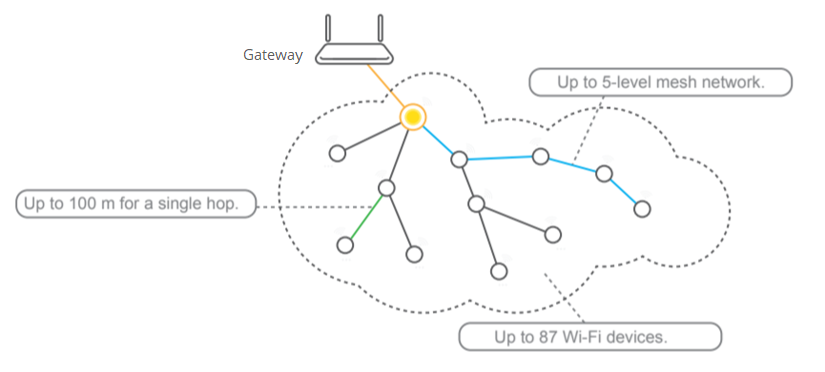
\includegraphics[width=\textwidth]{mesh.png}
  \caption{ESP8266 Mesh Network}
  \label{fig:mesh}
\end{figure}

WSNs make a large scale deployment of sensors economically viable for the farming domain \cite{pfWSN}. It supports many operations such as irrigation, fertilizer use, soil monitoring and intruder detection \cite{main3}. Its integration has resulted in a plethora of applications such as remote healthcare, water control, precision agriculture, smart cities, and wildlife monitoring \cite{main2}.

\section{Gateway}
An IoT gateway is a device/software that serves as the bridge between the WSN and the cloud side. It is responsible for device management, data processing, and routing \cite{usingGateways}.

\noindent
In a cloud-based network architecture, these gateways act as edge nodes, reducing the amount of processing power required on the cloud end. As seen in Figure~\ref{fig:gateway}, this reduces both the cost and the complexity of the network. 

\begin{figure}[h]
  \centering
  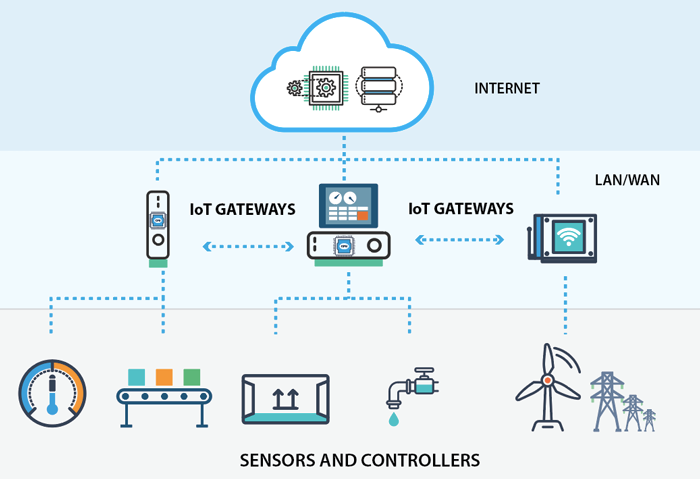
\includegraphics[width=0.9\textwidth]{gateway.png}
  \caption{Role of an IoT Gateway \cite{whatGateway}}
  \label{fig:gateway}
\end{figure}

\noindent
It performs several tasks on their behalf, such as: \cite{usingGateways}
\begin{itemize}
  \item Communicating with IoT Platform;
  \item Connecting to the internet when the device can't directly connect itself, such as a ZigBee or Bluetooth device;
  \item Providing secure authentication when the device can't send its credentials, or when you want to add a layer of security by using the credentials of both the device and the gateway;
  \item Publishing telemetry events, device management, getting configuration data, or setting device state;
  \item Storing and processing data, logs and telemetry; and
  \item Translating between different protocols.
\end{itemize}

